\scanpage{160}
$\unsure{r}\quad\deleted{\unsure{\varepsilon_0\varepsilon_0\widetilde\varepsilon_0}}$
\[
\widetilde\rho',\quad\widetilde\rho''=\sigma(\widetilde\rho')
\]
\figure{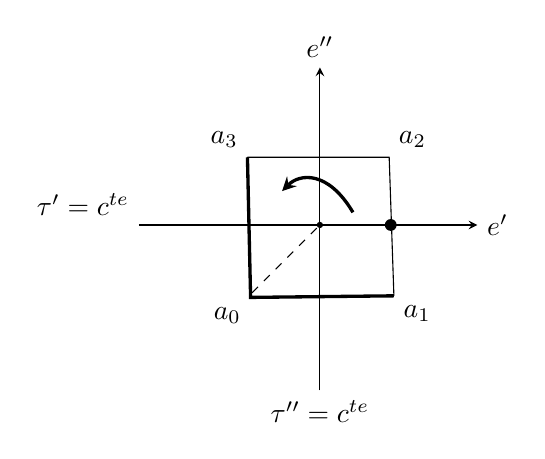
\begin{tikzpicture}[x=1cm,y=1cm,>=stealth]
\draw[->] (-2.3,0)--(2,0) node[right] {$e'$};
\draw[->] (0,-2.1)--(0,2) node[above] {$e''$};
\draw (-.92,.86)--(.88,.86)--(.94,-.9);
\draw[very thick] (-.92,.86)--(-.88,-.92)--(.94,-.9);
\draw[dashed] (-.86,-.86)--(0,0); \fill (0,0) circle (.04); \fill (.9,0) circle (.075);
\draw[->,very thick] (.42,.16) .. controls (.1,.7) and (-.26,.65) .. (-.48,.43);
\node[above left] at (-.92,.86) {$a_3$}; \node[above right] at (.88,.86) {$a_2$};
\node[below left] at (-.88,-.92) {$a_0$}; \node[below right] at (.94,-.9) {$a_1$};
\node[above left] at (-2.3,0) {$\tau'=c^{te}$}; \node[below] at (0,-2.1) {$\tau''=c^{te}$};
\end{tikzpicture}}
\[
\left\{\begin{array}{ll}
\tau'e'=e' & \tau''e'=-e'\\
\tau'e''=-e'' & \tau''e''=e''\\[.7em]
\sigma e'=e'' & \sigma e''=-e'
\end{array}\right.
\]
\[
\begin{gathered}
\tau'\tau''=\tau''\tau'=\sigma^2\deleted{\unsure{\infty}}=\omega_0\\
\sigma^4=\omega_0^2=1\\
\deleted{\unsure{\sigma\tau''=\tau''\sigma}}\\
\deleted{\unsure{\tau'\varepsilon_0}}
\end{gathered}
\]
\margin{$\left\{\begin{array}{l}\omega_0e'=-e'\\\omega_0e''=-e''\end{array}\right.$}
\[
\begin{array}{ll}
\sigma\tau'=\tau'_\infty=r_0 &: \quad e'\longmapsto e''\\
\Vert &\quad e''\mathrel{\mapstochar\relbar\relbar\mapstochar}e'\\
\tau'\sigma^{-1} &\\
\Vert &\\
\sigma^{-1}\tau''=\tau''\sigma&\\
(\tau'=\sigma^2\tau''&
\end{array}
\]
\[
\begin{array}{l}
\tau''\longmapsto\tau_\infty=r_\infty\\
\sigma\longmapsto\sigma=\sigma_\infty\\
\varepsilon'\longmapsto\varepsilon_0\\
\varepsilon''=\sigma(\varepsilon')\mathrel{\mapstochar\relbar\relbar\mapstochar}\varepsilon_1
\end{array}
\qquad
\begin{array}{l}
\varepsilon'(e')=e'\\
\varepsilon'e''=e''-e'
\end{array}
\]
\margin{$\varepsilon'$ était $\rho'$ avant}
\[
\begin{array}{l}
\varepsilon_0=\sigma\rho\quad\varepsilon_1=\rho\sigma\\
\varepsilon_1\varepsilon_0=-\rho^2=\rho^{-1}\\
\deleted{-\varepsilon_1\varepsilon_0=\omega_0\varepsilon_1\varepsilon_0=}
\end{array}
\qquad
\left\{\begin{array}{l}
\sigma(\varepsilon')=\varepsilon''\\
\tau'(\varepsilon')=\tau''(\varepsilon')=\varepsilon^{\prime-1}\\
\tau'(\varepsilon'')=\tau''(\varepsilon'')=\varepsilon^{\prime\prime-1}
\end{array}\right.
\]
\deleted{$\unsure{\varepsilon_0}\quad\varepsilon_1\varepsilon_0=\unsure{\rho_0}$}
\[
\left\{\begin{array}{l}
\rho=(\varepsilon_1\varepsilon_0)^{-1}=\varepsilon_0^{-1}\varepsilon_1^{-1}\\
\sigma_\infty=\varepsilon_0\rho^{-1}=\varepsilon_0\varepsilon_1\varepsilon_0=\rho^{-1}\varepsilon_1=\varepsilon_1\varepsilon_0\varepsilon_1\\
\deleted{\unsure{\tau_0}}\quad r_0(\varepsilon_0)=\varepsilon_1^{-1}\\
r_0(\varepsilon_1)=\varepsilon_0^{-1}
\end{array}\right.
\]
\margin{$\deleted{\unsure{\varepsilon_0\varepsilon_1}}$}
\[
\left[\begin{array}{l}
r_0(\rho)=\varepsilon_1\varepsilon_0=\rho^{-1}\\
r_0(\sigma)=\varepsilon_1^{-1}\varepsilon_0^{-1}\varepsilon_1^{-1}=\varepsilon_0^{-1}\varepsilon_1^{-1}\varepsilon_0^{-1}
\end{array}\right.
\]
\[
\varepsilon_0,\varepsilon_1,\unsure{\tau_0|r_0}
\]
\margin{i.e. $\begin{gathered}
\varepsilon_1\varepsilon_0\varepsilon_1=\varepsilon_0\varepsilon_1\varepsilon_0\\
\rho\sigma\sigma\rho\rho\sigma=\sigma\rho\rho\sigma\sigma\rho\\
\deleted{\unsure{\varepsilon_1\underbrace{\varepsilon_0\varepsilon_1\varepsilon_0\varepsilon_1^{-1}}_{\longleftarrow}\varepsilon_0^{-1}}}\\
\rho\sigma^2\rho^2\sigma=\sigma\rho^2\sigma^2\rho\\
-\underbrace{\rho^3\sigma}_{\sigma}=-\underbrace{\sigma\rho^3}_{\sigma}
\end{gathered}$}

\margin{160}
